\chapter{界面设计}
\section{客户端界面}

\subsection{PC 客户端界面} % (fold)
\label{sub:pc_客户端界面}

本小节讲述在PC客户端上,用户界面应具有的设计需求。

\begin{enumerate}
	\item \textbf{要求的屏幕格式}:
		PC客户端支持大于$800 \times 600$ 分辨率的屏幕,并对根据屏幕大小以及系统
		设定的屏幕元素放大比例做自动适应;
	\item \textbf{使用方式}:
		对于一般的用户,我们的产品使用逻辑与一般的PC软件一致,
			用户不需要主动学习便可学会使用它,
		同时,我们也会在安装后附上使用说明书,来保证用户可以方便使用;
	\item \textbf{页面规划}: 
	\begin{itemize}
		\item 主页界面的用户界面设计,请参考图\ref{fig:desttop_home};
		\item 音乐播放界面的用户界面设计,请参考图\ref{fig:desttop_music};
		\item 音乐集查看界面的用户界面设计,请参考图\ref{fig:desttop_collection};
	\end{itemize}
\end{enumerate}

\newpage
\begin{figure}[h!]
  \centering

  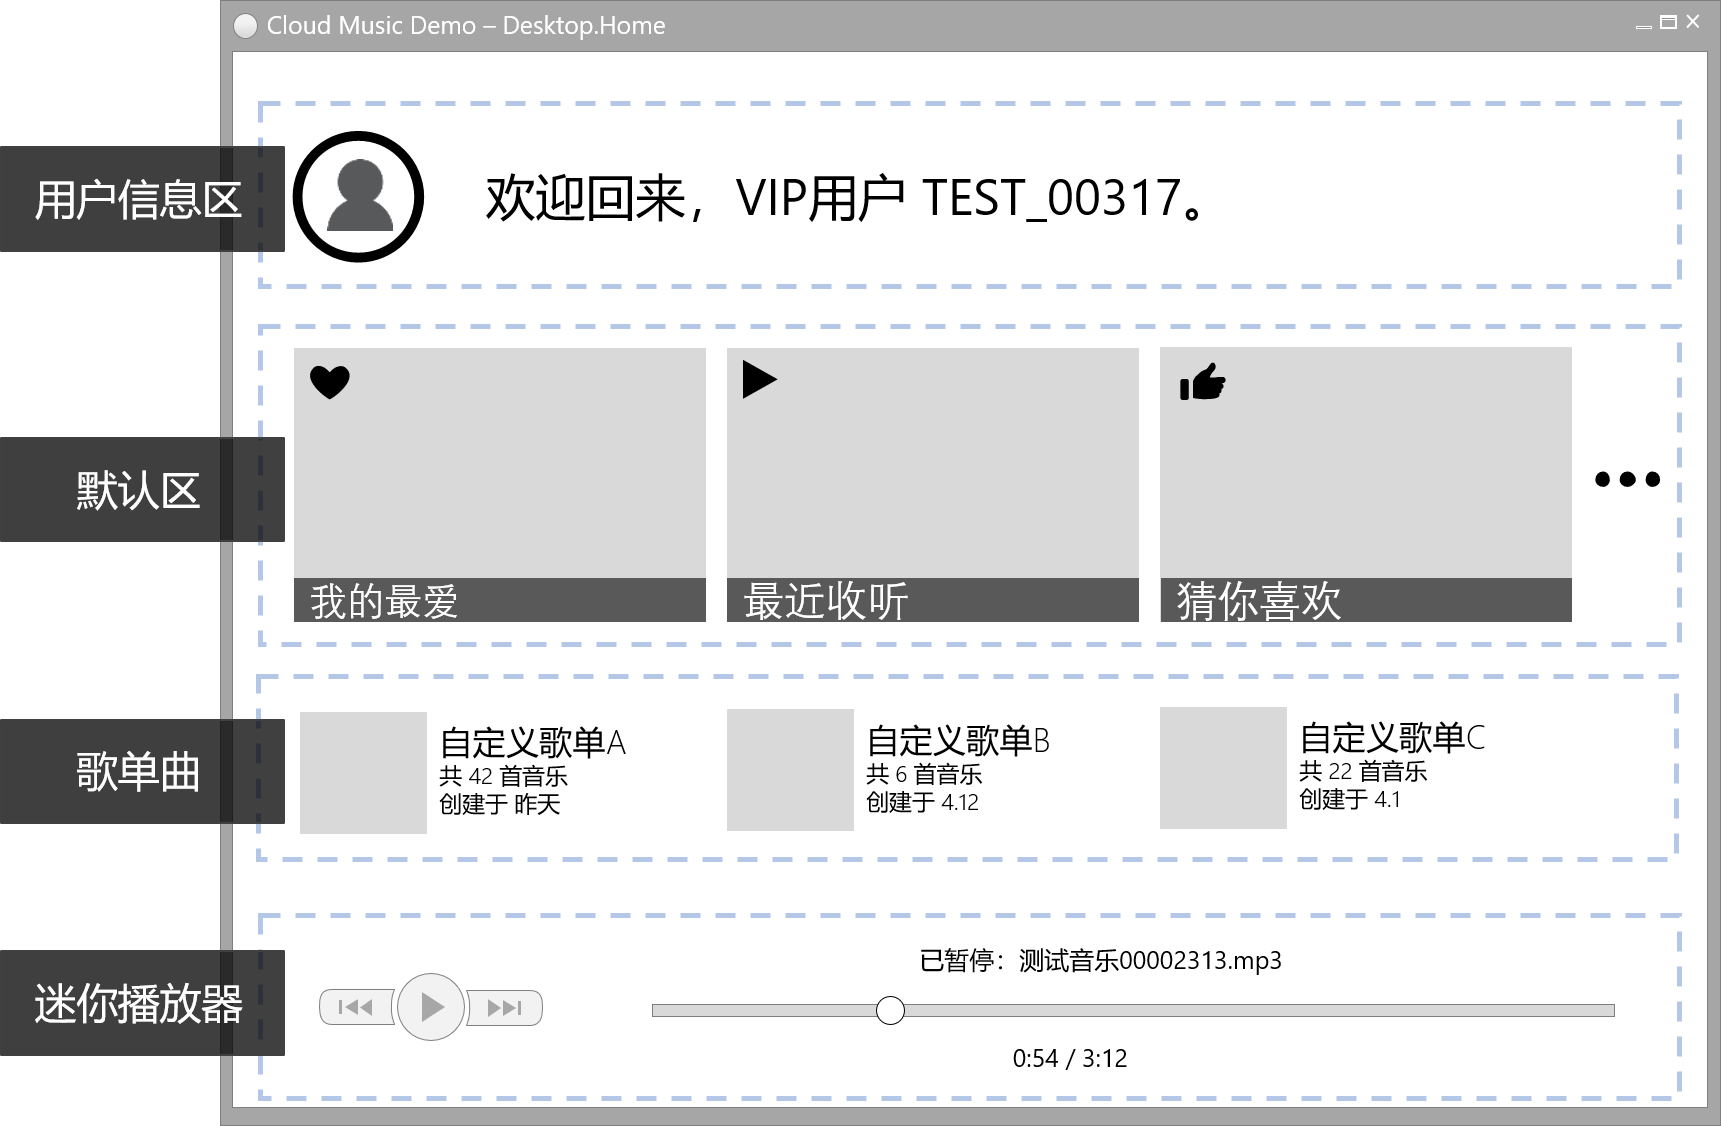
\includegraphics[width=.95\linewidth]{figures/desttop_home}

  \caption{  \label{fig:desttop_home}
  		PC客户端主页(Home Page)用户界面设计图
    }
\end{figure}

\begin{figure}[h!]
  \centering
 
  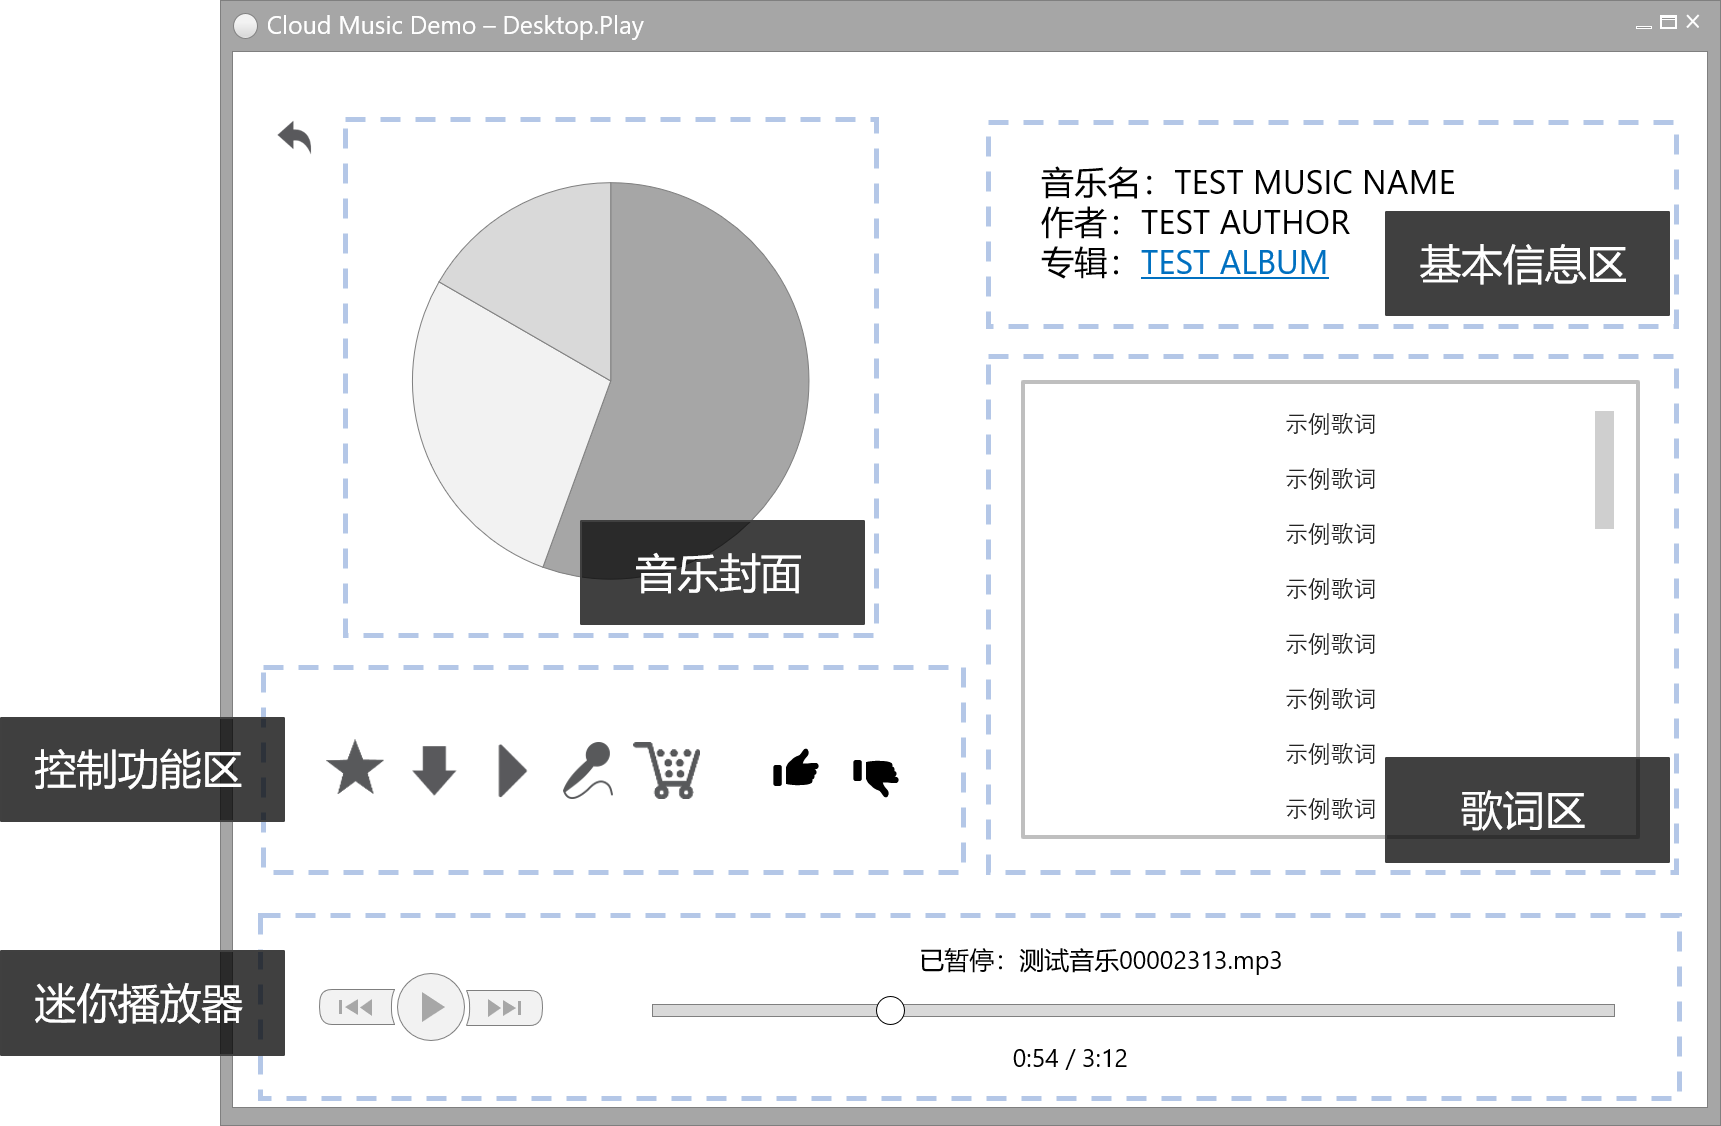
\includegraphics[width=.95\linewidth]{figures/desttop_music}

  \caption{ \label{fig:desttop_music}
  		PC客户端音乐播放界面用户界面设计图
    }
\end{figure}

\newpage
\begin{figure}[h!]
  \centering

  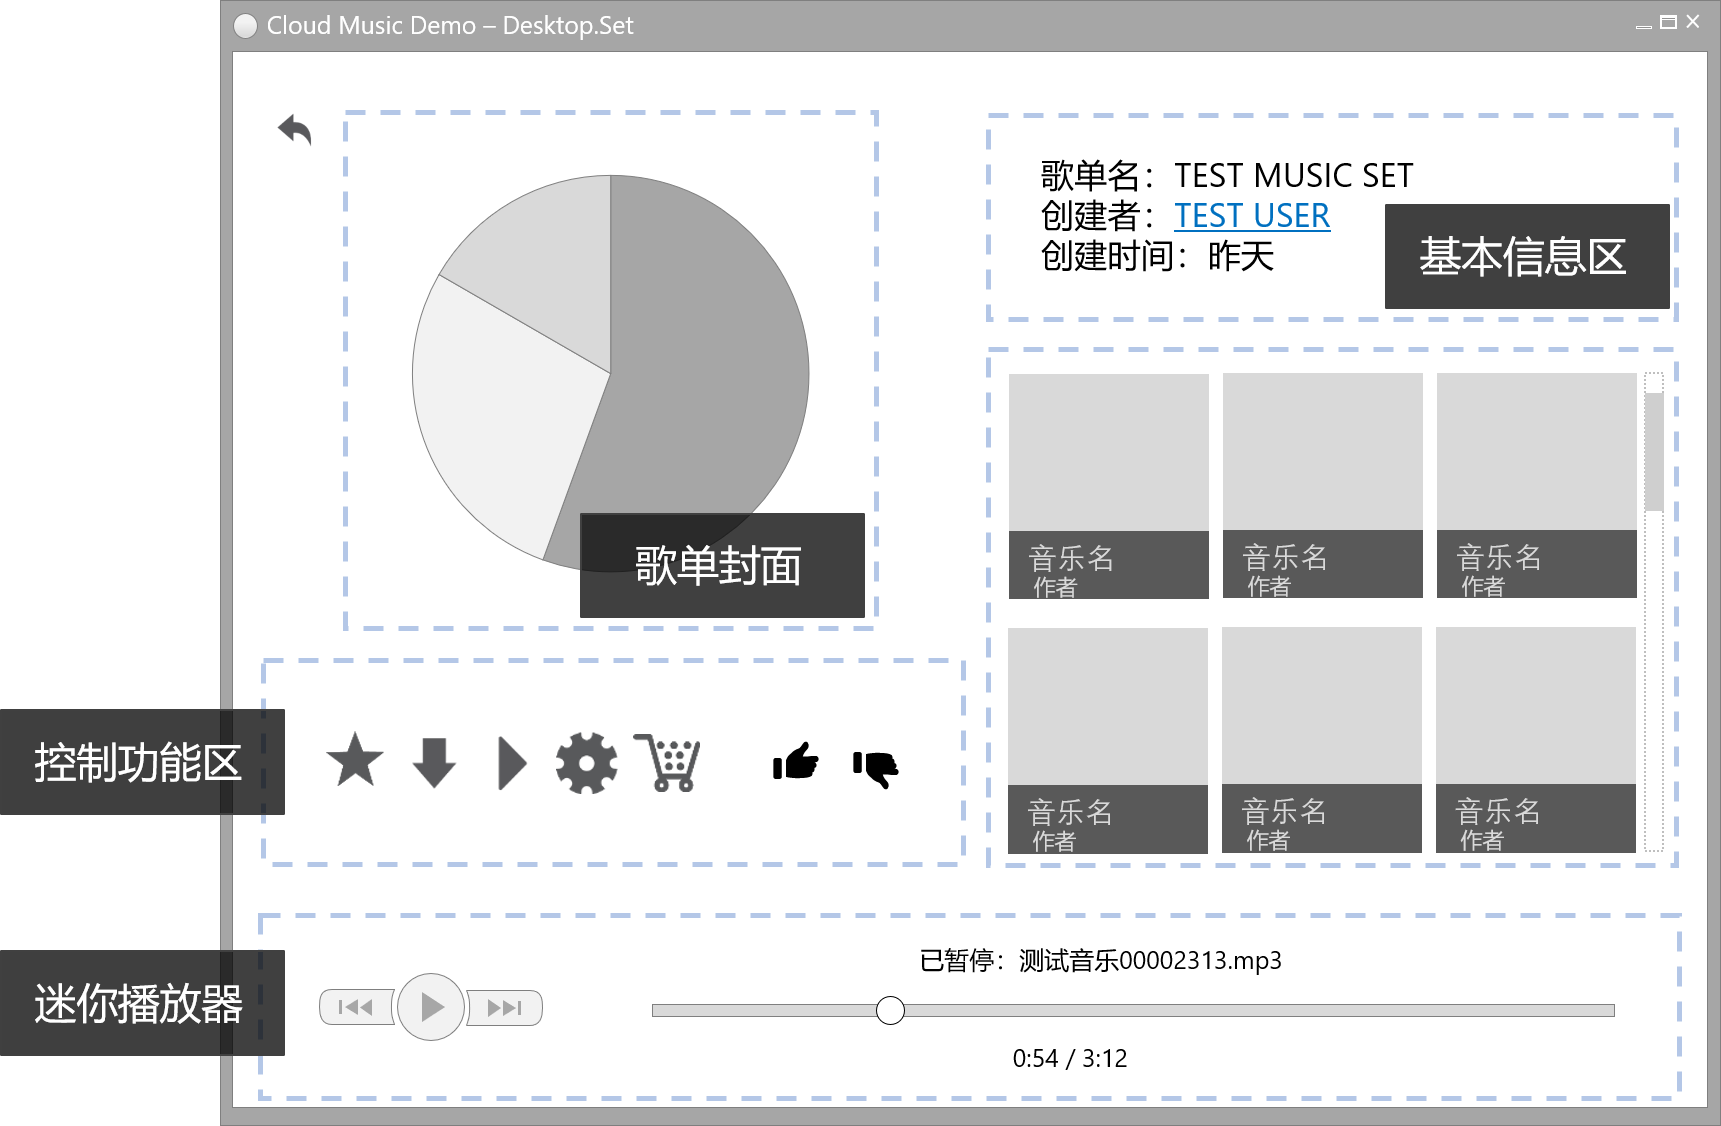
\includegraphics[width=.95\linewidth]{figures/desttop_collection}

  \caption{  \label{fig:desttop_collection}
  		PC客户端音乐集展示用户界面设计图
    }
\end{figure}

% subsection pc_客户端界面 (end)
\subsection{移动客户端界面} % (fold)
\label{sub:移动客户端界面}
\begin{enumerate}
	\item \textbf{要求的屏幕格式}:
		PC客户端支持大于$1334 \times 750$ 分辨率的移动设备屏幕,并对根据屏幕大小以及系统
		设定的屏幕元素放大比例做自动适应;
	\item \textbf{使用方式}:
		对于一般的用户,我们的产品使用逻辑与一般的移动设备软件一致,
			用户不需要主动学习便可学会使用它,
		同时,我们也会在安装后附上使用说明书,来保证用户可以方便使用;
	\item \textbf{页面规划}: 
	\begin{itemize}
		\item 主页界面的用户界面设计,请参考图\ref{fig:mobile_home};
		\item 音乐播放界面的用户界面设计,请参考图\ref{fig:mobile_music};
		\item 音乐集查看界面的用户界面设计,请参考图\ref{fig:mobile_collection};
	\end{itemize}
\end{enumerate}

\begin{figure}[h!]
  \centering

  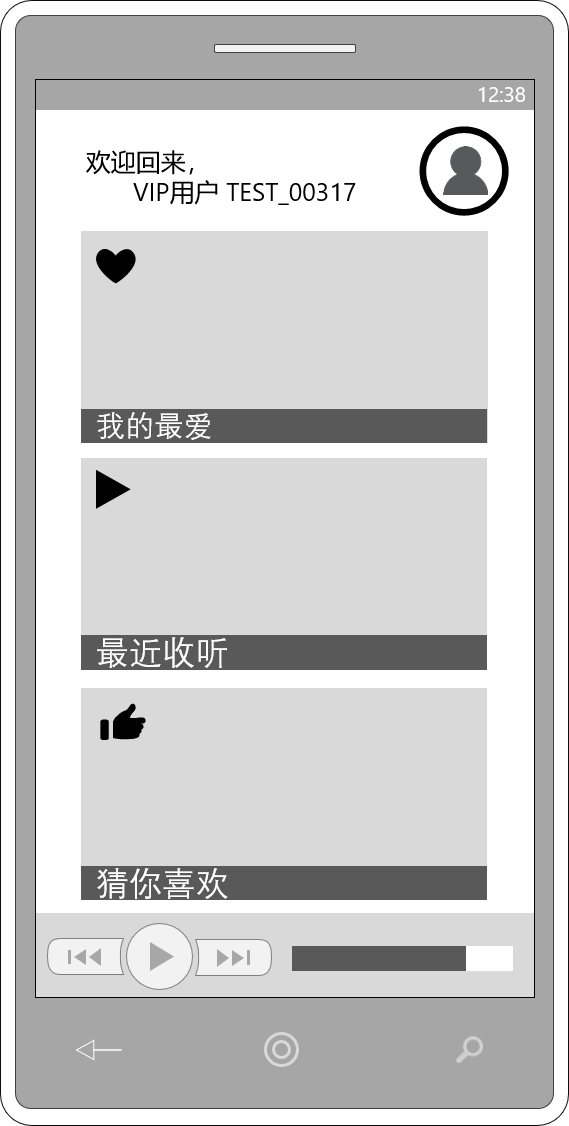
\includegraphics[width=.33\linewidth]{figures/mobile_home}

  \caption{  \label{fig:mobile_home}
  		移动客户端主页(Home Page)用户界面设计图
    }
\end{figure}

\begin{figure}[h!]
  \centering
 
  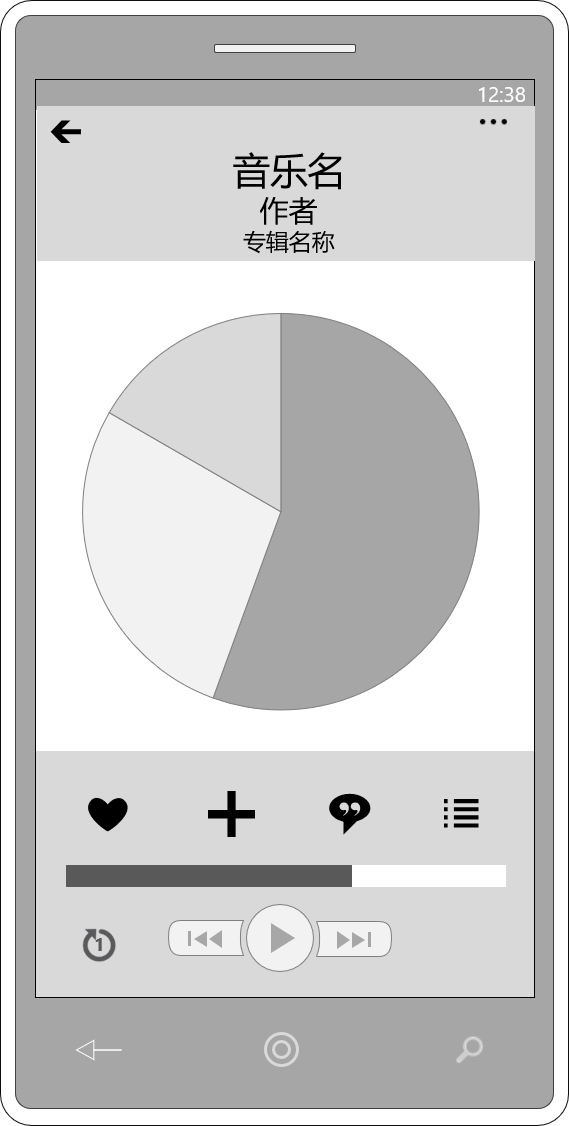
\includegraphics[width=.33\linewidth]{figures/mobile_music}

  \caption{ \label{fig:mobile_music}
  		移动客户端音乐播放界面用户界面设计图
    }
\end{figure}

\begin{figure}[h!]
  \centering

  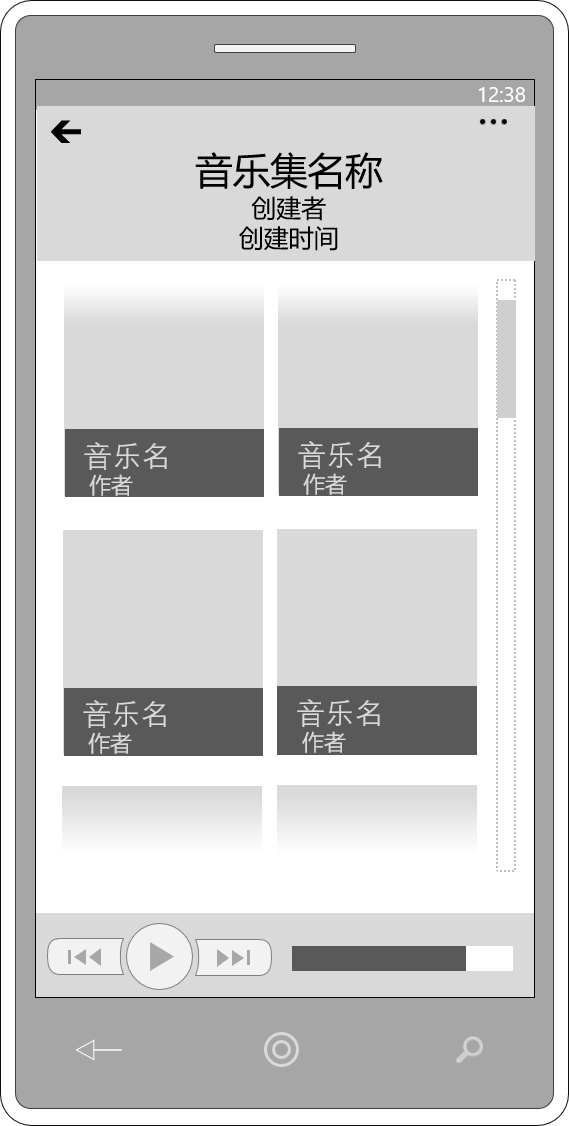
\includegraphics[width=.33\linewidth]{figures/mobile_collection}

  \caption{  \label{fig:mobile_collection}
  		移动客户端音乐集展示用户界面设计图
    }
\end{figure}
% subsection 移动客户端界面 (end)

\newpage
\subsection{网页客户端用户界面} % (fold)

\begin{enumerate}
	\item \textbf{要求的屏幕格式}:
		网页客户端支持大于$800 \times 600$ 分辨率的通用网页浏览器,
		并对根据屏幕大小以及浏览器设定的屏素放大比例做自动适应;
	\item \textbf{使用方式}:
		对于一般的用户,我们的产品使用逻辑与一般的网页一致,
			用户不需要主动学习便可学会使用它,
		同时,我们也会在安装后附上使用说明书,来保证用户可以方便使用;
	\item \textbf{页面规划}: 
	\begin{itemize}
		\item 主页界面的用户界面设计,请参考图\ref{fig:web_home};
		\item 音乐播放界面的用户界面设计,请参考图\ref{fig:web_music};
		\item 音乐集查看界面的用户界面设计,请参考图\ref{fig:web_collection};
	\end{itemize}
\end{enumerate}

\begin{figure}[h!]
  \centering

  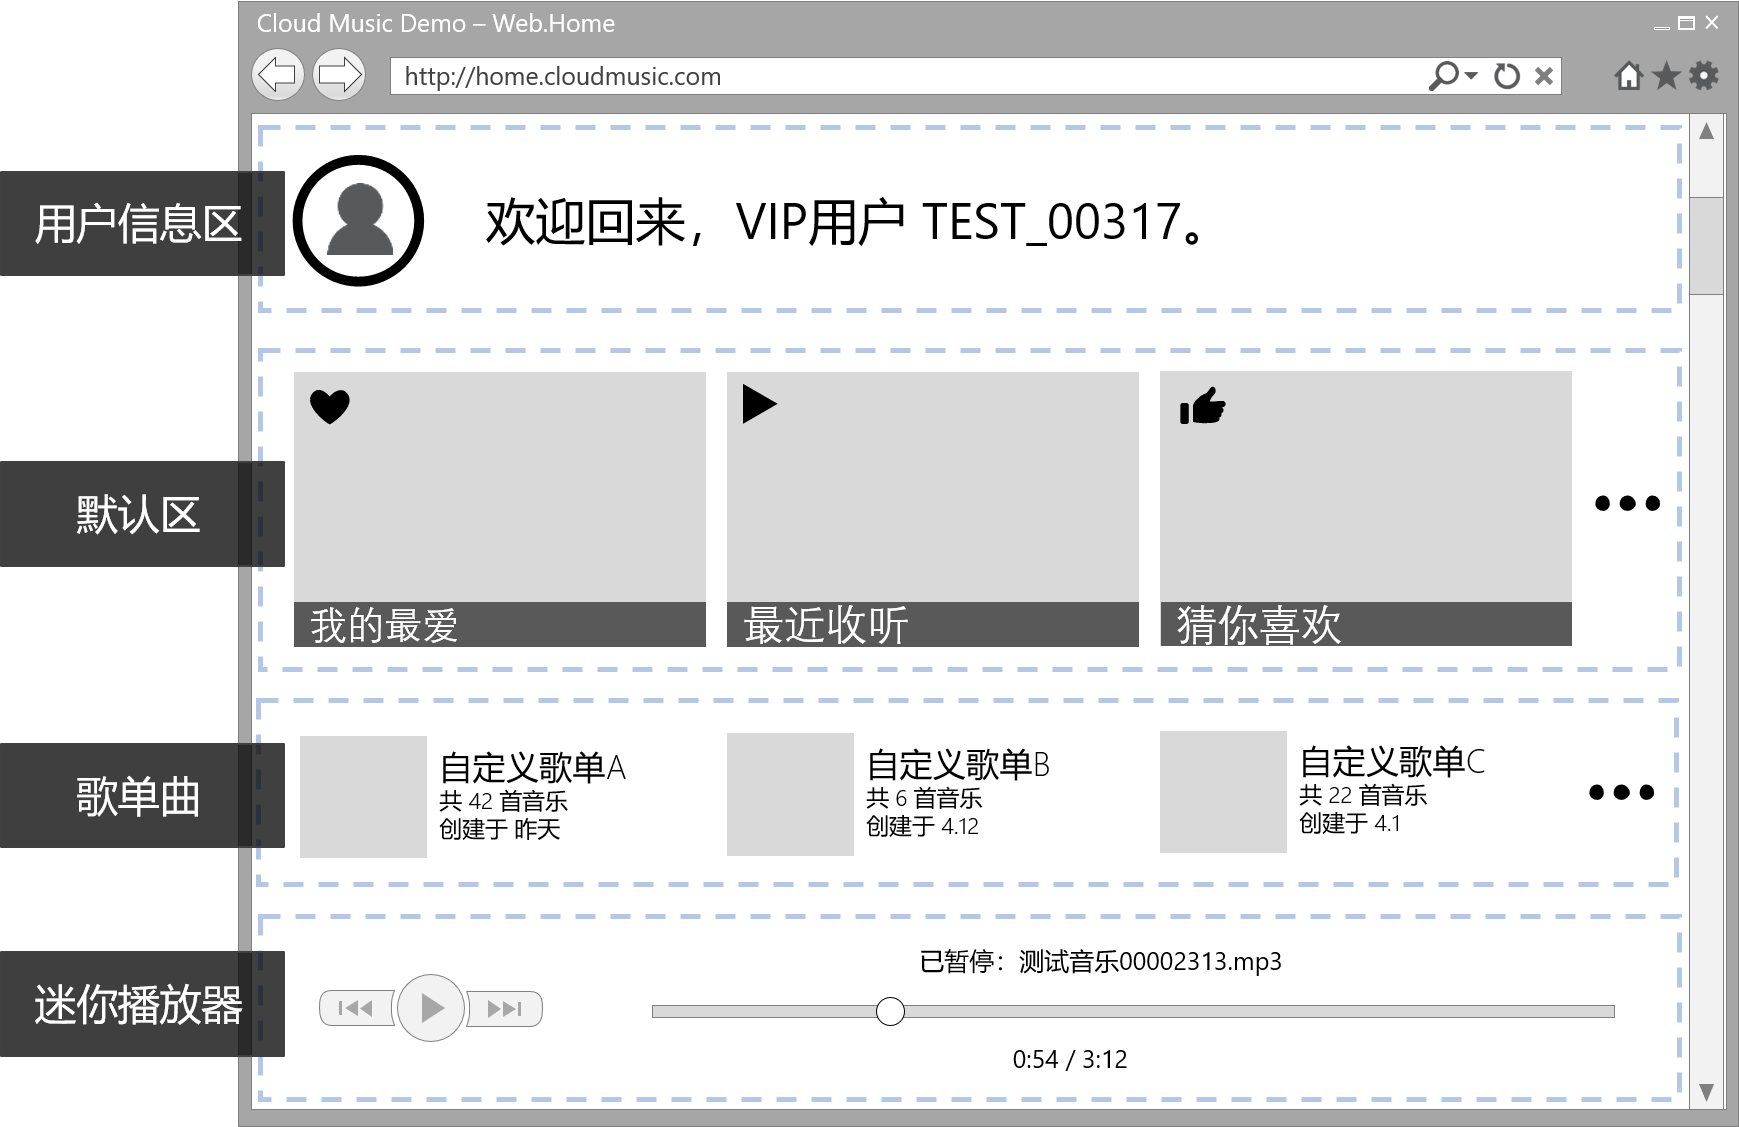
\includegraphics[width=.99\linewidth]{figures/web_home}

  \caption{  \label{fig:web_home}
  		网页客户端主页(Home Page)用户界面设计图
    }
\end{figure}

\begin{figure}[h!]
  \centering
 
  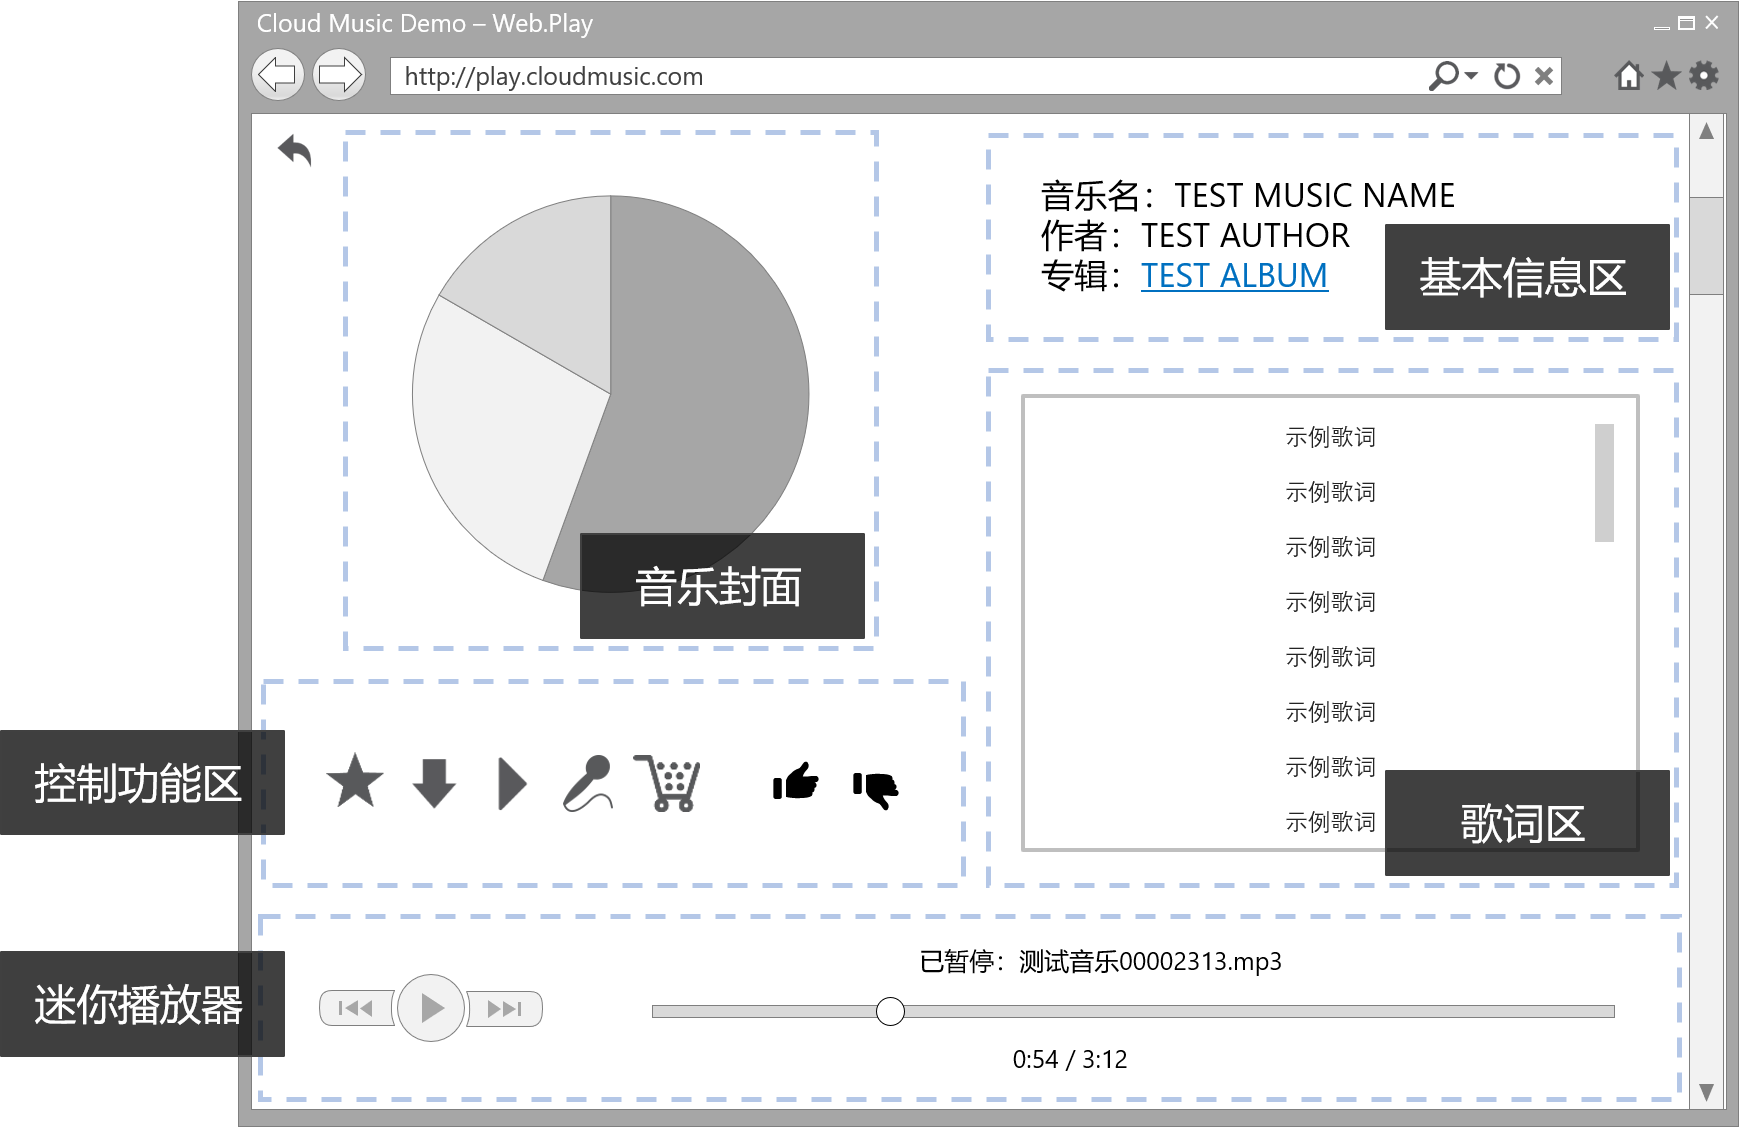
\includegraphics[width=.99\linewidth]{figures/web_music}

  \caption{ \label{fig:web_music}
  		网页客户端音乐播放界面用户界面设计图
    }
\end{figure}

\begin{figure}[h!]
  \centering

  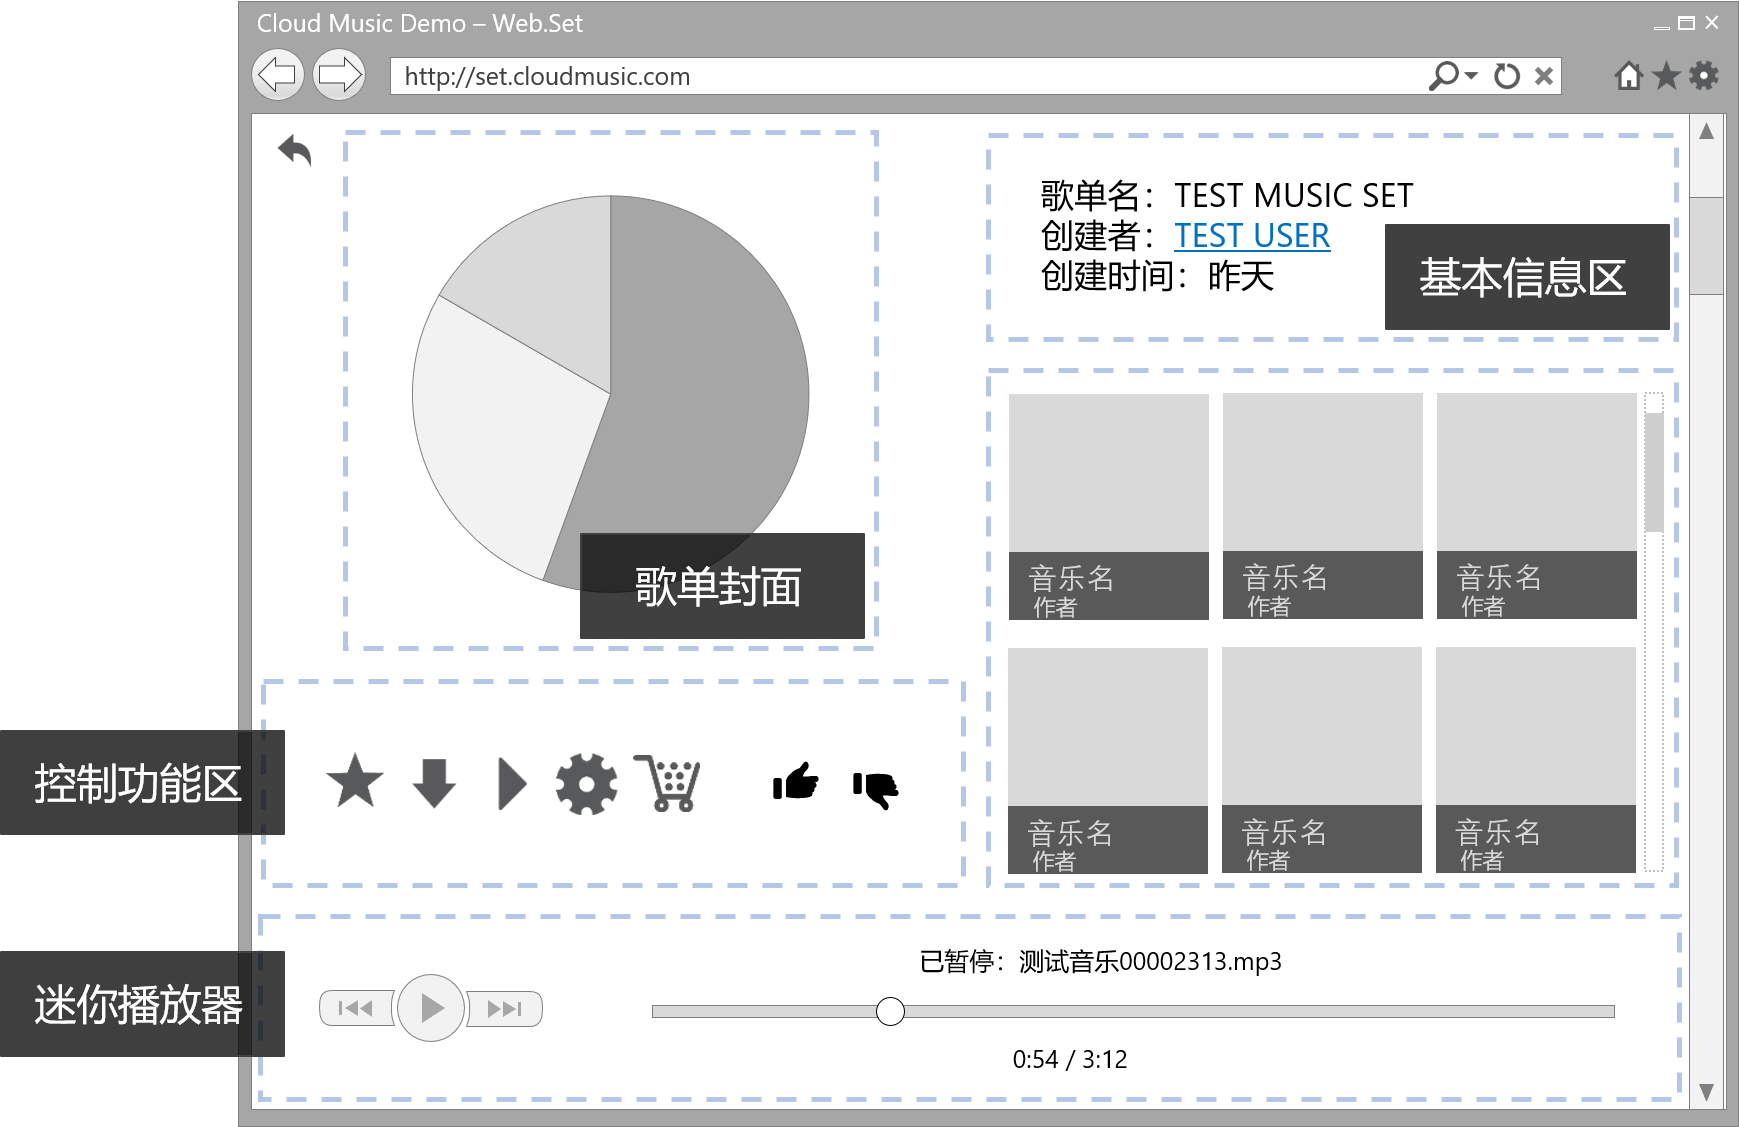
\includegraphics[width=.99\linewidth]{figures/web_collection}

  \caption{  \label{fig:web_collection}
  		网页客户端音乐集展示用户界面设计图
    }
\end{figure}
\newpage
\section{服务器端界面}
\begin{enumerate}
	\item \textbf{要求的屏幕格式}:
		服务器端仅支持在内部网页上,支持大于$800 \times 600$ 分辨率的通用网页浏览器,
		并对根据屏幕大小以及浏览器设定的屏素放大比例做自动适应;
	\item \textbf{使用方式}:
		对于管理员,我们的产品使用逻辑与一般的网页一致,
			管理员不需要主动学习便可学会使用它,
		同时,我们也会在安装后附上使用说明书,来保证管理员可以方便使用;
	\item \textbf{页面规划}: 
	\begin{itemize}
		\item 管理界面的用户界面设计,请参考图\ref{fig:sudo};
	\end{itemize}
\end{enumerate}

\begin{figure}[h!]
  \centering

  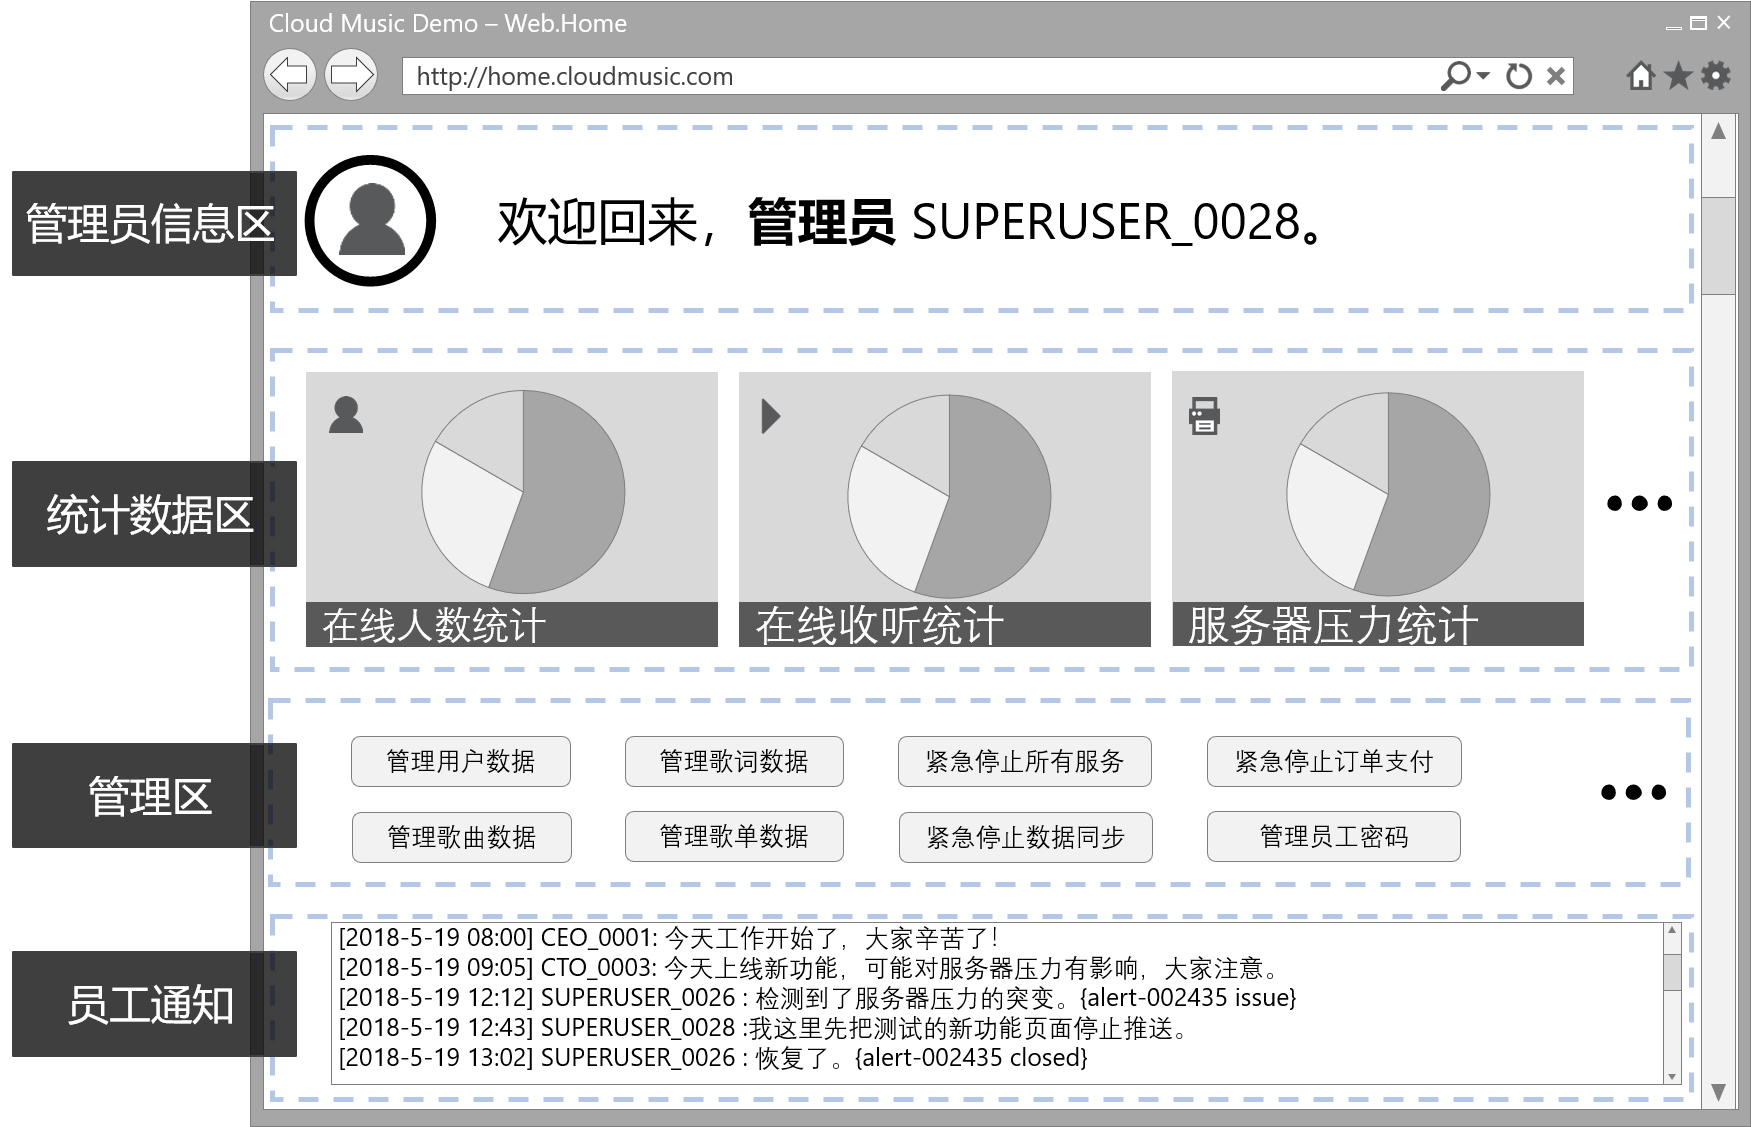
\includegraphics[width=.99\linewidth]{figures/sudo}

  \caption{  \label{fig:sudo}
  		服务端管理界面的用户界面设计图
    }
\end{figure}